\section{Configuration}

\subsection{Common}

\subsubsection{Main}

\begin{figure}[H]
    \center
      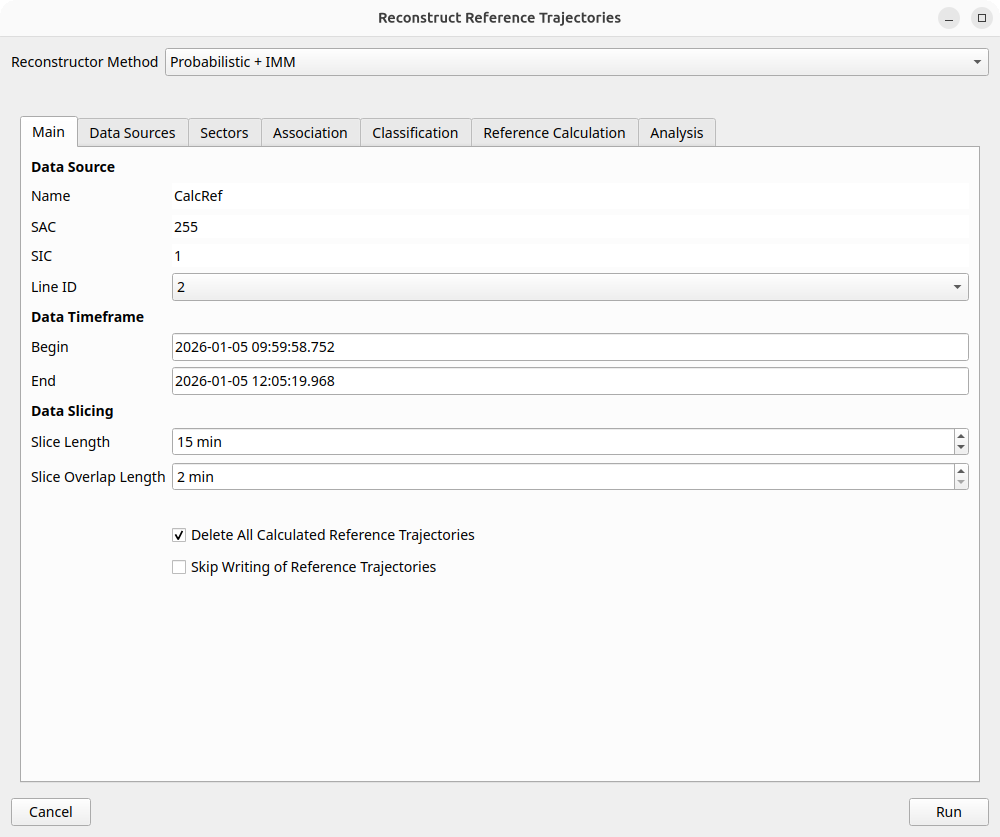
\includegraphics[width=16cm,frame]{figures/dialog_main.png}
    \caption{Calculate References Main}
\end{figure}

In the main tab, the following parameters can be set:

\begin{itemize}
\item Data Source: Data source to be created for calculated references
    \begin{itemize}
    \item Name, SAC, SIC: Data source parameters
    \item Line ID: Line ID to be used
    \end{itemize}
\item Data Timeframe: Time window of data to be processed
    \begin{itemize}
    \item Begin / End timestamps
    \end{itemize}
\item Data Slicing: Time slice sizes
    \begin{itemize}
    \item Slice Length: Duration of a time slice
    \item Slice Overlap Length: Duration of an overlap region to "glue" slices together
    \end{itemize}
\item Delete All Calculated Reference Trajectories: If active, all previous calculated references are deleted
\item Skip Writing of Reference Trajectories: If active, calculated references and associations are not written into the database
\end{itemize}
\ \\

\subsubsection{Data Sources}

\begin{figure}[H]
    \center
      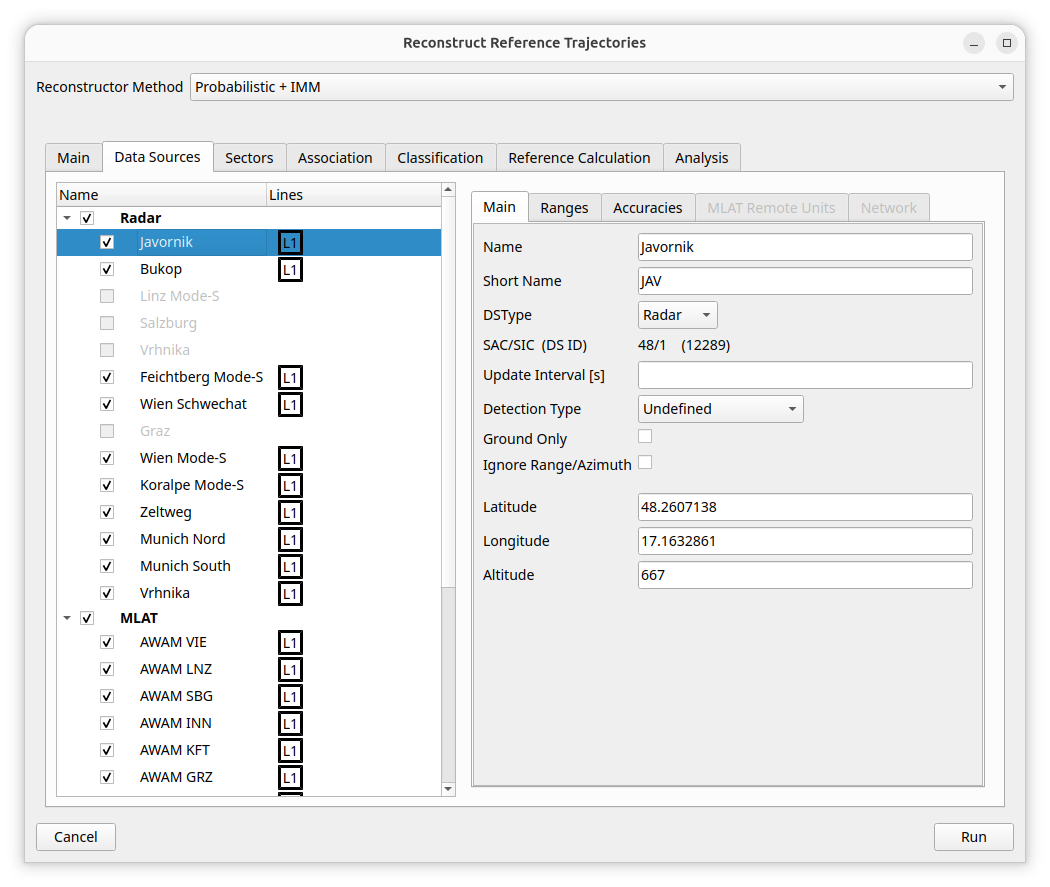
\includegraphics[width=16cm,frame]{figures/dialog_data_sources.png}
    \caption{Calculate References Data Sources}
\end{figure}

In this tab, the data sources to contribute to the calculated references can be selected. \\

Please \textbf{note} that de-selected data sources are still associated, but only their target report positions do not contribute to the references. \\

Please also \textbf{note} that for ground surveillance datasets containing \textbf{SMRs}, it is imperative to set both the detection type to "Primary Only", as well as to set the "Ground Only" checkbox. Otherwise, SMR plots will be associated over long distances and cause sub-optimal reconstructor results.

\subsubsection{Classification}

In the classification, special parameters can be set to identify the AnyAircraft and Vehicle categories. Any target (without any other class information) and any Mode C code above the given 'Minimum Aircraft Altitude' will be classified as AnyAircraft. Vehicles (without any other class information) can be set by giving a list of Mode S Aircraft Identification and/or Aircraft Addresses. \\

\begin{figure}[H]
    \center
      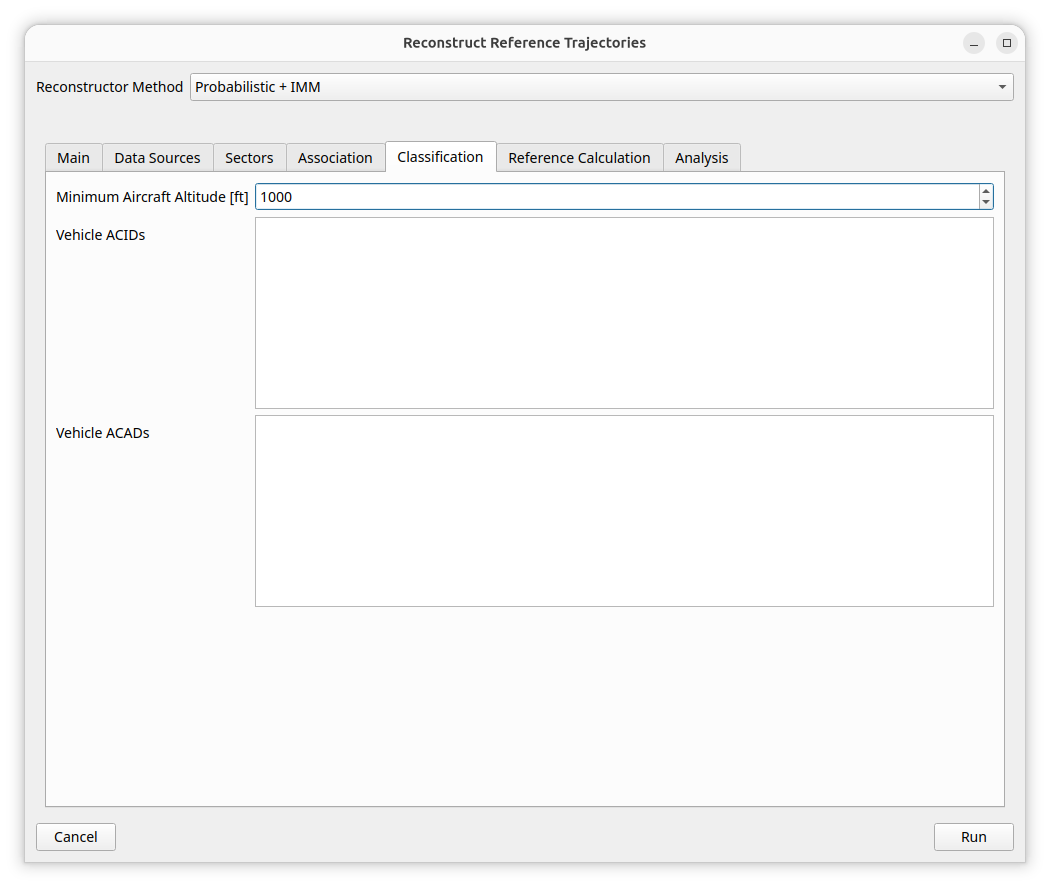
\includegraphics[width=16cm,frame]{figures/dialog_class.png}
    \caption{Classification Parameters}
\end{figure}

\subsection{Scoring + UMKalman Parameters}

\subsubsection{Association}

\begin{figure}[H]
    \center
      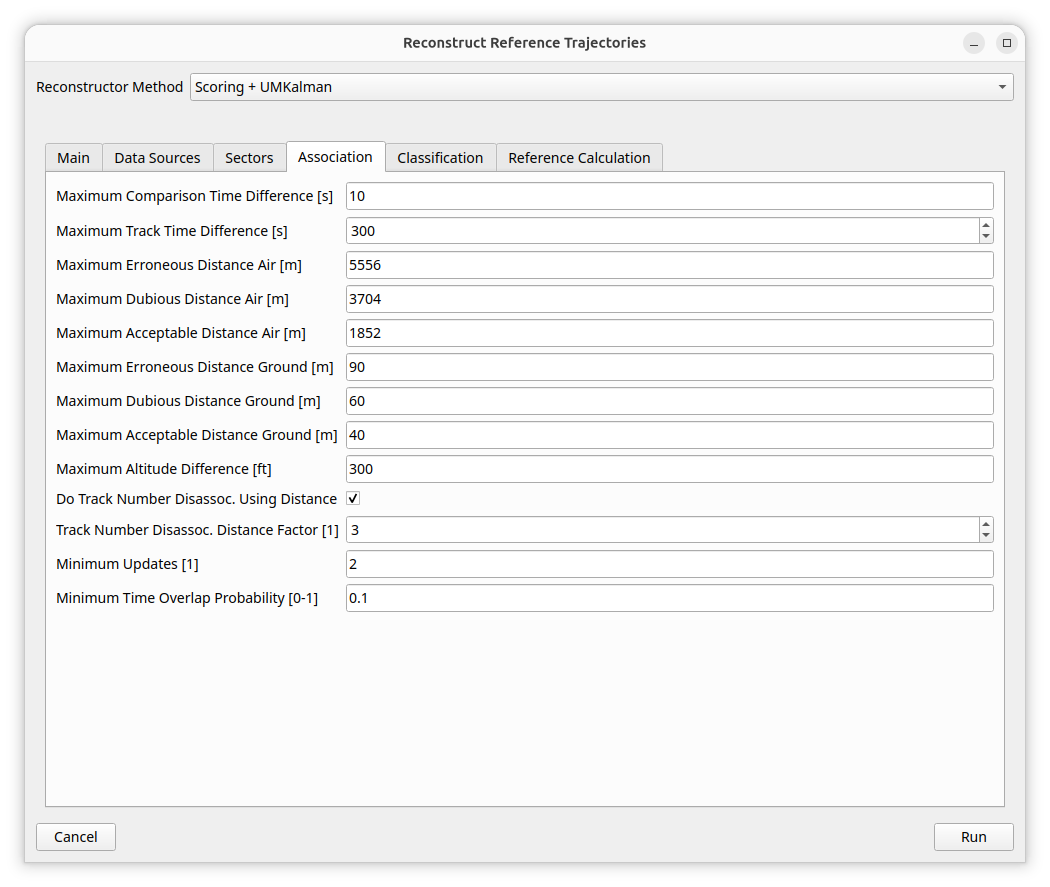
\includegraphics[width=16cm,frame]{figures/dialog_scorum_assoc.png}
    \caption{Scoring + UMKalman Association Parameters}
\end{figure}

In this tab, the association parameters can be set, i.e. the thresholds used to associate target reports to targets, or targets to targets. \\

\begin{table}[H]
  \center
  \begin{tabularx}{\textwidth}{ | l | l | l | X |}
    \hline
    \textbf{Parameter} & \textbf{Unit} & \textbf{Default} &  \textbf{Description} \\ \hline
    Maximum Comparison Time Difference & s & 10 & Maximum time delta for any code/position comparison \\ \hline 
    Maximum Track Time Difference & s & 300 & Maximum time delta to a previously associated track \\ \hline
    
    Maximum Erroneous Distance Air & m & 5556 (3nm) & Target/target association \\ \hline
    Maximum Dubious Distance Air & m & 3704 (2nm) & Target/target association \\ \hline
    Maximum Acceptable Distance Air & m & 1852 (1nm)& Target/target association \\ \hline
    
    Maximum Erroneous Distance Ground & m & 90 & Target/target association \\ \hline
    Maximum Dubious Distance Ground & m & 60 & Target/target association \\ \hline
    Maximum Acceptable Distance Ground & m & 40 & Target/target association \\ \hline
    
    Maximum Altitude Difference & ft & 300 & Maximum altitude difference \\ \hline
    Do Track Number Disassoc. Using Distance & & true & Whether to disassociate track numbers from targets based on position \\ \hline
    Track Number Disassoc. Distance Factor & 1 & 3$\sigma$ & Maximum number of standard deviations distance \\ \hline
    Minimum Updates & 1 & 2 & Target/target association \\ \hline
    Minimum Time Overlap Probability & 1 & 0.1 & Target/target association \\ \hline
  \end{tabularx}
\end{table}
\ \\
\hl{TODO explain this shit, llimit Pram size}

The following table lists the configuration parameters available for the Scoring + UMKalman reconstructor (Simple Reconstructor) related to association.

\begin{table}[H]
    \centering
    \footnotesize
    \hspace*{-1.5cm}
    \begin{tabular}{|p{4.5cm}|p{6.5cm}|l|l|l|}
    \hline
    \textbf{Parameter Name} & \textbf{Description} & \textbf{Complexity} & \textbf{Default} & \textbf{Range} \\ \hline
    Maximum Comparison Time Difference & Maximum interpolation window for associating a report to a track. & Advanced & 6.0 s & 0.1 -- 60 s \\ \hline
    Maximum Track Time Difference & Maximum time gap to resume an existing track using its data source track number. & Intermediate & 300 s & 60 -- 3600 s \\ \hline
    Maximum Erroneous Distance Air & Distance limit rejecting position matches (Air). & Intermediate & 9260 m & 500 -- 10000 m \\ \hline
    Maximum Dubious Distance Air & Threshold for Dubious classification (Air). & Intermediate & 3704 m & 250 -- 25000 m \\ \hline
    Maximum Acceptable Distance Air & Threshold for Acceptable classification (Air). Typically 1-2 NM or less. & Intermediate & 1852 m & 50 -- 10000 m \\ \hline
    Maximum Erroneous Distance Ground & Distance limit rejecting position matches (Ground). & Intermediate & 90 m & 70 -- 200 m \\ \hline
    Maximum Dubious Distance Ground & Threshold for Dubious classification (Ground). & Intermediate & 60 m & 30 -- 100 m \\ \hline
    Maximum Acceptable Distance Ground & Threshold for Acceptable classification (Ground). & Intermediate & 40 m & 10 -- 50 m \\ \hline
    Maximum Altitude Difference & Max. diff. in Mode C altitude for association. & Basic & 300 ft & 0 -- 5000 ft \\ \hline
    Do Track Number Disassoc. Using Distance & If enabled, matching track numbers are rejected if spatial distance is too large. & Basic & True & True/False \\ \hline
    Track Number Disassoc. Distance Factor & Multiplier of Acceptable Distance to validate track number reuse. & Advanced & 3 & 1 -- 20 \\ \hline
    Minimum Updates & Minimum updates to validate a target or confirm a merge. & Intermediate & 2 & $\ge 1$ \\ \hline
    Minimum Time Overlap Probability & Minimum time overlap probability for merging similar targets. & Advanced & 0.1 & 0.05 -- 0.9 \\ \hline
    \end{tabular}
    \caption{Configuration parameters for the Scoring + UMKalman Reconstructor}
    \label{tab:reconst_simple_params}
\end{table}

\subsubsection{Reference Calculation}
\label{sec:reconst_scorum_ref_calc} 

\begin{figure}[H]
    \center
      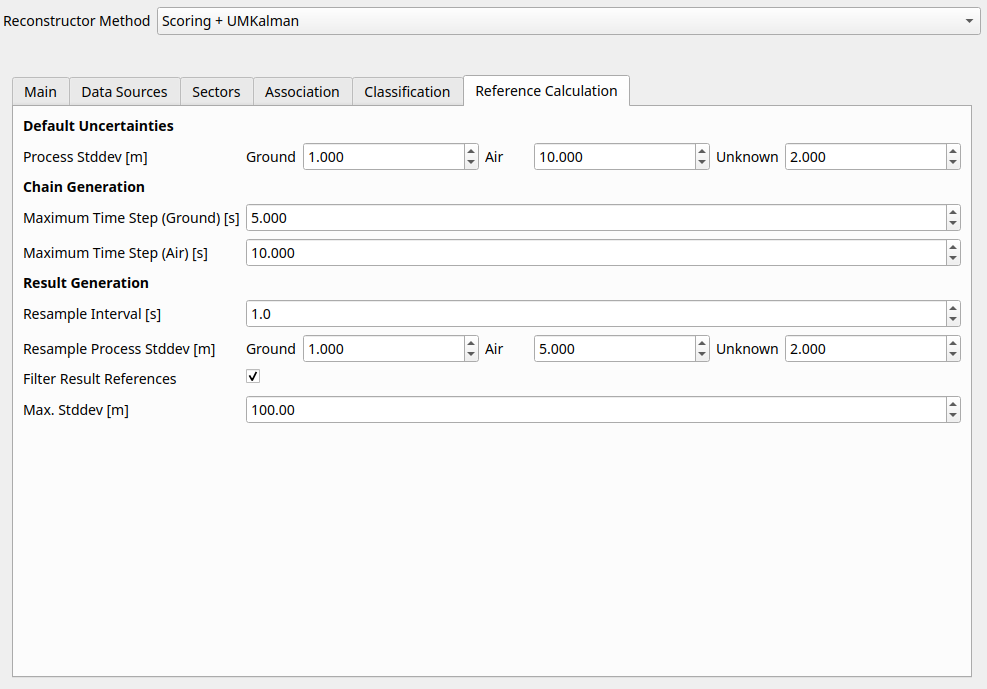
\includegraphics[width=16cm,frame]{figures/dialog_ref_calc.png}
    \caption{Scoring + UMKalman Reference Calculation Parameters}
\end{figure}

In this tab, the reference calculation parameters can be set, i.e. the Kalman and reconstruction parameters used for position estimation of the references. \\

\begin{table}[H]
  \center
  \begin{tabularx}{\textwidth}{ | l | l | l | X |}
    \hline
    \textbf{Parameter} & \textbf{Unit} & \textbf{Default} &  \textbf{Description} \\ \hline
    Process Stddev Ground & m & 3 & Process noise for ground targets \\ \hline
    Process Stddev Air & m & 7 & Process noise for FL400 targets \\ \hline
    Process Stddev Unknown & m & 5 & Process noise for targets w/o altitude \\ \hline
    Maximum Time Step (Ground) & s & 5 & Re-init reference if no update available within given time (on ground) \\ \hline
    Maximum Time Step (Air) & s & 10 & Re-init reference if no update available within given time (in air) \\ \hline
    Resample Interval & s & 1 & Update interval for the resampled reference trajectories \\ \hline
    Resample Process Stddev Ground & m  & 2 & Resampling process noise for ground targets \\ \hline
    Resample Process Stddev Air & m & 5 & Resampling process noise for FL400 targets \\ \hline
    Resample Process Stddev Unknown & m  & 3 & Resampling process noise for targets w/o altitude \\ \hline    
    Filter Result References & & true & Whether to filter written reference trajectory updates based on maximum position standard deviation \\ \hline
    Max. Stddev & m & 100 & Maximum position standard deviation \\ \hline
  \end{tabularx}
\end{table}

The following table lists the configuration parameters available for the Scoring + UMKalman reconstructor related to reference trajectory calculation (Kalman filtering).

\begin{table}[H]
    \centering
    \footnotesize
    \hspace*{-1.5cm}
    \begin{tabular}{|p{4.5cm}|p{6.5cm}|l|l|l|}
    \hline
    \textbf{Parameter Name} & \textbf{Description} & \textbf{Complexity} & \textbf{Default} & \textbf{Range} \\ \hline
    Process Stddev (Ground) & Assumed process noise standard deviation for targets on ground (affects maneuverability allowance). & Basic & 5.0 m & $>0$ m \\ \hline
    Process Stddev (Air) & Assumed process noise standard deviation for airborne targets. & Basic & 10.0 m & $>0$ m \\ \hline
    Process Stddev (Unknown) & Assumed process noise standard deviation for targets with unknown state. & Basic & 7.0 m & $>0$ m \\ \hline
    Maximum Time Step (Ground) & Maximum time interval between updates used for interpolation/prediction on ground. & Intermediate & 5.0 s & $>0$ s \\ \hline
    Maximum Time Step (Air) & Maximum time interval between updates used for interpolation/prediction in air. & Intermediate & 10.0 s & $>0$ s \\ \hline
    Resample Interval & Time interval for the output trajectory (if resampling enabled internally). & Basic & 2.0 s & 0.1 -- 30 s \\ \hline
    Resample Process Stddev (Ground) & Process noise applied specifically during the resampling phase for ground targets. & Advanced & 2.0 m & $>0$ m \\ \hline
    Resample Process Stddev (Air) & Process noise applied specifically during the resampling phase for airborne targets. & Advanced & 5.0 m & $>0$ m \\ \hline
    Resample Process Stddev (Unknown) & Process noise applied during resampling for unknown state targets. & Advanced & 3.0 m & $>0$ m \\ \hline
    Filter Result References & Enable filtering of the final reference trajectory based on estimated accuracy (Standard Deviation). & Intermediate & False & True/False \\ \hline
    Max. Stddev & Maximum allowed position standard deviation for a point to be included in the final reference. & Intermediate & 150.0 m & $>0$ m \\ \hline
    \end{tabular}
    \caption{Reference Calculation parameters for the Scoring + UMKalman Reconstructor}
    \label{tab:reconst_simple_ref_params}
\end{table}

Result resampling is enabled in order to obtain reference trajectories with a homogeneous sample rate. 
It is carried out by interpolating the Kalman states at fixed time-steps. The accuracy of the resulting samples
follows the Kalman accuracies more closely when interpolating near the endpoints of a segment, and it will decrease
in the middle of a segment. The amount of decrease of accuracy will depend on the time duration of the segment and the used 
process standard deviation (parameter \textit{Resample Process Stddev}).

\subsection{Probabilistic + IMM Parameters}

\subsubsection{Association}

\begin{figure}[H]
    \center
      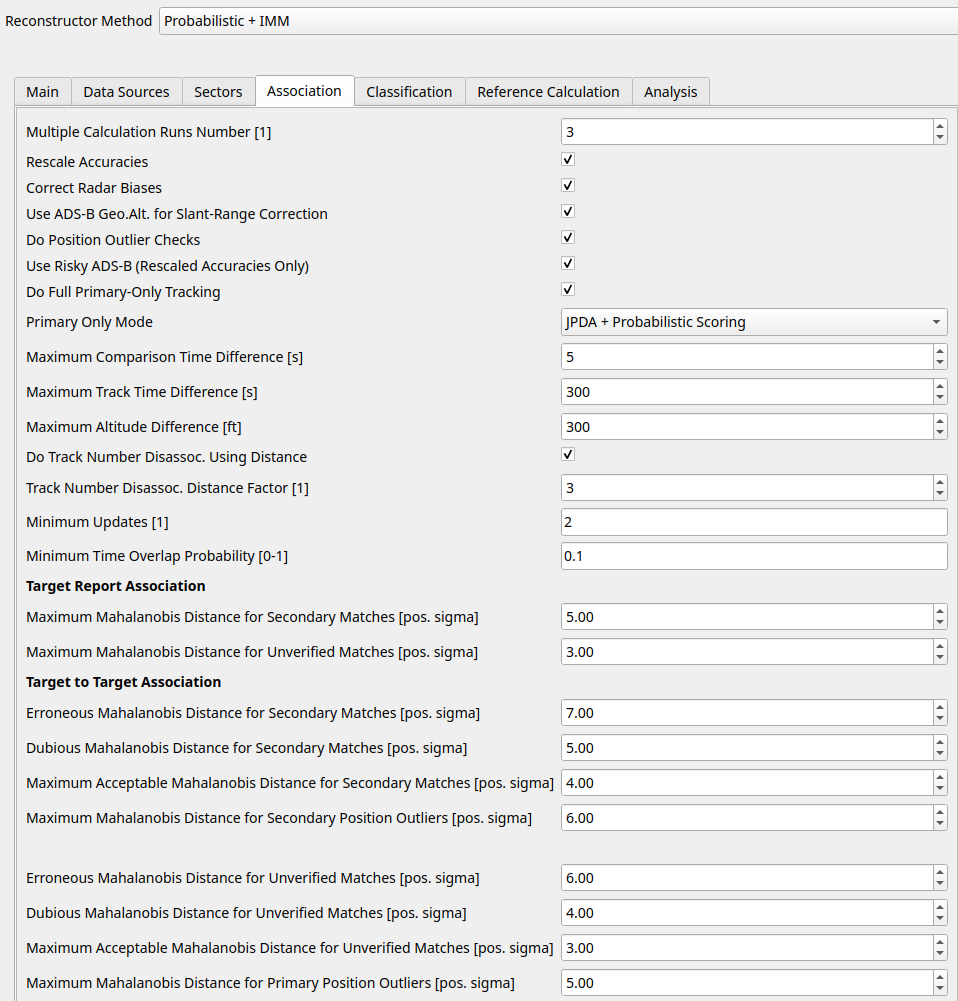
\includegraphics[width=17cm,frame]{figures/dialog_probimm_assoc.png}
    \caption{Probabilistic + IMM Association Parameters}
\end{figure}

\textbf{JPDA}

\begin{figure}[H]
    \center
      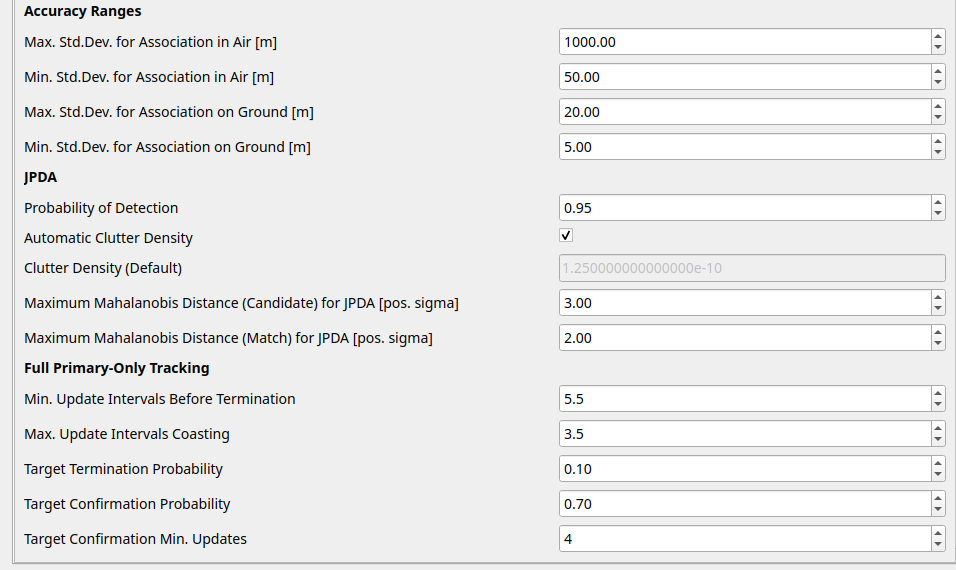
\includegraphics[width=16cm,frame]{figures/dialog_probimm_assoc_jpda.png}
    \caption{Probabilistic + IMM Association Parameters}
\end{figure}


Please \textbf{note} that a detailed discussion of the given parameters can be found in the section \nameref{sec:appendix_reconstructor}  .

\subsubsection{Reference Calculation}

\begin{figure}[H]
    \center
      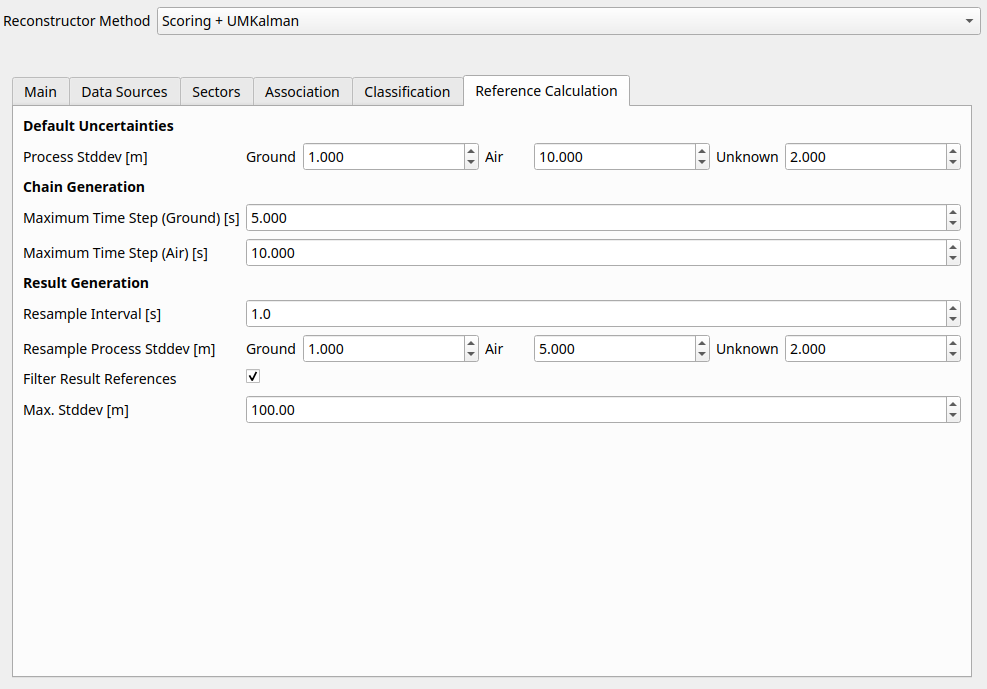
\includegraphics[width=16cm,frame]{figures/dialog_ref_calc.png}
    \caption{Probabilistic + IMM Reconstruction Parameters}
\end{figure}

The given parameters are the same as discussed in the 'Scoring + UMKalman' chapter, please refer to \nameref{sec:reconst_scorum_ref_calc} for details.

\subsubsection{Analysis}

\begin{figure}[H]
    \center
      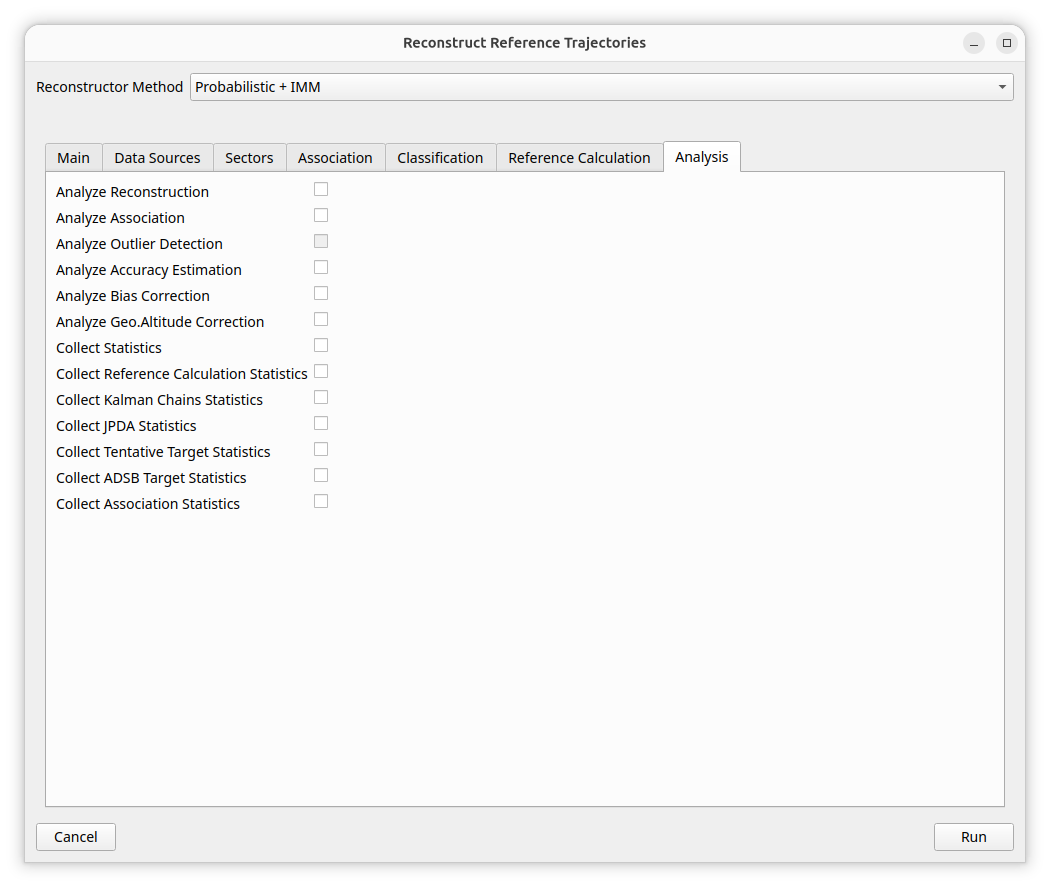
\includegraphics[width=16cm,frame]{figures/dialog_probimm_analyse.png}
    \caption{Probabilistic + IMM Analysis Parameters}
\end{figure}

Please \textbf{note} that a detailed discussion of the given parameters is out of scope for this user manual. For users with a professional license, a dedicated reconstructor user manual appendix is provided.
